\begin{graphicspathcontext}{{./chapters/mas/imgs/},{./chapters/mas/imgs/auto/},\old}

\begin{frame}{Agent: a first definition}
	\begin{definitionblock}{Agent \cite{Wooldridge09}}
		An agent is an entity with (at least) the following attributes/characteristics:
		\begin{enumerate}
		\item Autonomy
		\item Interaction - Social Skills - Sociability
		\item Reactive behavior
		\item Proactive behavior
		\end{enumerate}
	\end{definitionblock}
	\vspace{.5cm}	
	\hiconbox*{No commonly/universally accepted definition}{info-icon}
\end{frame}

\begin{frame}[t]{Agent: Autonomy}
	\begin{columns}
		\begin{column}{.2\linewidth}
			\begin{bottomarrowsequence}
				\arrow[bg=CIADgreen]{Autonomy}
				\arrow{Interaction}
				\arrow{Reactive}
				\arrow{Proactive}
			\end{bottomarrowsequence}
		\end{column}
		\begin{column}{.8\linewidth}
			\begin{definitionblock}{Principle of autonomy}
				Agents encapsulate their \Emph{internal state} (that is not accessible to other agents), and make decisions about what to do based on this state, without the direct intervention of humans or others agent
			\end{definitionblock}
			\vspace{.5cm}
			\begin{itemize}
				\item Able to \alert{act without any direct intervention} of human users or other agents
				\item Total \alert{control} over its own \alert{internal state}
				\item Total \alert{control} over its own \alert{actions} (no master/slave relationship)
				\item Can modify its behavior according to its experience (\alert{adaptation} or \alert{learning})
			\end{itemize}
		\end{column}
	\end{columns}
\end{frame}

\begin{frame}[t]{Agent: Interaction}
	\vspace{-.5cm}
	\begin{columns}
		\begin{column}[t]{.2\linewidth}
			\begin{bottomarrowsequence}
				\arrow{Autonomy}
				\arrow[bg=CIADgreen]{Interaction}
				\arrow{Reactive}
				\arrow{Proactive}
			\end{bottomarrowsequence}
		\end{column}
		\begin{column}[t]{.8\linewidth}
			\only<1>{
				\begin{definitionblock}{Principle of interaction}
					Agent interacts with other agents, and have the ability to engage in social activities (cooperation, coordination, negotation...) in order to achieve its goals
				\end{definitionblock}
				\begin{itemize}
				\item \Emph{The whole is greater than the sum of its parts}
				\item Require a mechanism to exchange information
				\item Many tasks can only be done by:
					\begin{description}
					\item[Cooperation] Agents work together toward a shared goal, often by sharing resources or information to achieve mutual benefit
					\item[Coordination] Agents organize their actions and interactions to avoid conflicts, ensure efficiency, and align with system objectives
					\item[Negotiation] Agents engage in communication and bargaining to resolve conflicts, allocate tasks, or reach agreements on actions or resource use
					\end{description}
				\end{itemize}
			}
			\only<2->{
				\begin{columns}
					\begin{column}[t]{.5\linewidth}
						\fancybox[width=5.2cm]{Direct Interaction}{
							\Emph{Peer-to-peer communication} \\
							Direct, bilateral, and explicit addressing
						}{direct-agent-interaction}{}
					\end{column}
					\begin{column}[t]{.5\linewidth}
						\fancybox[width=5.7cm]{Indirect Interaction}{
							\Emph{Stigmergy: interact without direct contact through the environment} \\
							Deposit persistent traces,
							Perceive and react to traces
						}{indirect-agent-interaction}{}
					\end{column}
				\end{columns}
				\begin{center}
					\only<2>{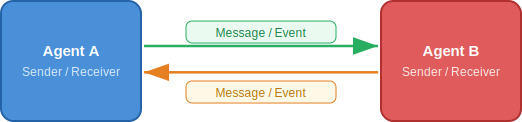
\includegraphics[width=.6\linewidth]{direct_interaction}}
					\only<3>{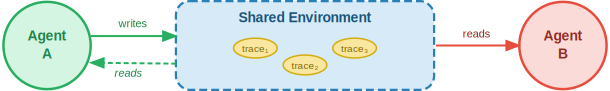
\includegraphics[width=.7\linewidth]{indirect_interaction}}
				\end{center}
			}
		\end{column}
	\end{columns}
\end{frame}

\begin{frame}[t]{Agent: Reactive Behavior}
	\vspace{-.5cm}
	\begin{columns}
		\begin{column}[t]{.2\linewidth}
			\begin{bottomarrowsequence}
				\arrow{Autonomy}
				\arrow{Interaction}
				\arrow[bg=CIADgreen]{Reactive}
				\arrow{Proactive}
			\end{bottomarrowsequence}
		\end{column}
		\begin{column}[t]{.8\linewidth}
			\begin{definitionblock}{Principle of reactive behavior}
				Agent \Emph{perceives} its environment and \Emph{immediately produces an action in response}, without planning or memory
			\end{definitionblock}
			\begin{description}
			\item[Perception $\rightarrow$ Action] behavior is a direct mapping from sensed stimuli to output actions
			\item[No internal model] agent holds no representation of the world
			\item[No deliberation] no reasoning, planning, or goal inference occurs
			\item[Quick response] reaction is immediate and computationally lightweight
			\item[Emergence] complex collective behaviors can arise from many simple reactive agents
			\end{description}
		\end{column}
	\end{columns}
\end{frame}

\begin{frame}[t]{Agent: Proactive Behavior}
	\vspace{-.5cm}
	\begin{columns}
		\begin{column}[t]{.2\linewidth}
			\begin{bottomarrowsequence}
				\arrow{Autonomy}
				\arrow{Interaction}
				\arrow{Reactive}
				\arrow[bg=CIADgreen]{Proactive}
			\end{bottomarrowsequence}
		\end{column}
		\begin{column}[t]{.8\linewidth}
			\begin{definitionblock}{Principle of proactive behavior}
				Agent \Emph{pursues its own goals} by anticipating future states and planning actions, independently of immediate stimuli
			\end{definitionblock}
			\begin{description}
			\item[Goal-driven] behavior is directed by internal objectives, not just external stimuli
			\item[Internal model] agent maintains a representation of the world to reason about it
			\item[Deliberation] agent evaluates options and selects actions toward its goals
			\item[Anticipation] agent predicts future states to plan ahead
			\item[Initiative] the agent acts on its own, without waiting for external triggers
			\end{description}
		\end{column}
	\end{columns}
\end{frame}

\sidenote{\cite{Ferber.1999,Weyns05,Michel.07}, Claude Sonnet 4.6}
\figureslide{{Agent and Agent Environment} in Multiagent Systems}{agentenvironment}

\begin{frame}[t]{{Some Questions} about the Agent Environment}
	\vspace{-.1cm}
	\begin{center}
		\begin{bottomarrowsequence}
			\arrow[bg=CIADlightgray,fg=CIADdarkgray]{What is included in the agent environment?}
			\arrow[bg=CIADdarkgray,fg=white]{Are all agent situated in the agent environment?}
			\arrow[bg=black,fg=white]{What is the the body of the agent and where is it localized?}
		\end{bottomarrowsequence}
	\end{center}
\end{frame}

\sidecite{Saunier2015}
\figureslide{Agent Body}{body_mind}

\begin{frame}{Agent: another definition}
	\footnotesize{
		\begin{definitionblock}{Agent \cite{Ferber.1999}}
			Agent is a virtual (software) or physical entity which:
			\begin{itemize}
			\item is capable of acting in an environment
			\item can communicate directly with other agents
			\item is driven by a set of tendencies (in the form of individual objectives or of a satisfaction/survival function which it tries to optimize)
			\item possesses resources of its own
			\item is capable to perceive its environment, but up to a limited extent
			\item has only a partial representation of this environment and perhaps none at all
			\item possesses skills and can offer services
			\item may be able to reproduce itself
			\item whose behavior tends towards satisfying its objectives, taking account of the resources and skills available to it and depending on its perception, its representation and the communication it receives
			\end{itemize}
		\end{definitionblock}
	}
\end{frame}

\begin{frame}{{Other Properties} for Agents}
	\smaller
	\begin{stabularx}{c|X|c}
	\tabularhead{Property}{Explanation}{Reference} \\
	Mobility & Move through different nodes of a network/grid & \tiny\cite{OKeefe98} \\
	\hline
	Adaptability & Modify the actions/behavior according to external conditions and perceptions & \tiny\cite{Weiss.99} \\
	\hline
	Versatility & Ability to perform different tasks or to meet different objectives & \tiny\cite{roadmapagentresearchdevel} \\
	\hline
	Trustiness & Level of confidence that inspires the agent to delegate tasks, perform action, collaborate with other agents & \tiny\cite{Sabater05} \\
	\hline
	Robustness & Continue to operate in fault situations, even with lower performances & \tiny\cite{Shehory98} \\
	\hline
	Persistence & Keep continuously running by retrieving or saving their internal state even after a crash or unexpected situations & \tiny\cite{Weiss.99} \\
	\hline
	Altruism & Disposition of an agent to assist other agents in their tasks & \tiny\cite{Castelfranchi98} \\
	\end{stabularx}
\end{frame}

%\begin{frame}{Agent vs. Object}
%	\begin{block}{Agent vs Object~\cite{Wooldridge.01.survey}}
%		\begin{itemize}
%		\item Agents are autonomous, they decide on the execution of services: ``\alert{\textit{Objects do it for free; agents do it because they want to}}''.
%		\item The agents allow flexible (reactive, pro-active, social) and autonomous behavior.
%		\item MAS are inherently ``multi-thread''. Each agent has its own thread of execution.
%		\end{itemize}
%	\end{block}
%\end{frame}



%\begin{frame}{Agent vs. Expert System}
%	\begin{block}{Key Differences}
%		An Expert System (ES) maintains various \alert{facts} about the world that are used to draw \alert{conclusions}.
%	\end{block}

%	\begin{block}{Key Differences}
%		\begin{itemize}
%		\item Traditional ES are not situated in an environment. There is no direct coupling with the environment and requires a user that acts as an intermediary ue.
%		\item ES are usually not capable of exhibiting flexible behavior (reactive and proactive).
%		\item ES are usually not provided with social skills (communication and interaction with other agents).
%		\end{itemize}
%	\end{block}
%\end{frame}

\end{graphicspathcontext}

\endinput

